\chapter{REST Api} % (fold)
\label{cha:rest_api}
\section{Architektura} % (fold)
\label{sec:architektura}
% section architektura (end)
\paragraph{} % (fold)
\label{par:}
\textit{REST}, czyli Represential State Transfer jest wzorcem opartym na doświadczeniach z tworzenia protokołu \textit{HTTP 1.0}. W dzisiejszych czasach \textit{REST} stał się dominującym modelem do projektowania usług sieci WEB. Opiera się na czterech głównych metodach znanych z protokołu \textit{HTTP}: 

\begin{itemize}
	\item GET - pobieranie daych,
	\item POST - tworzenie danych,
	\item PUT - modyfikowanie danych,
	\item DELETE - usuwanie danych.
\end{itemize}

\paragraph{} % (fold)
\label{par:}
Systemy w tej architekturze składają się z przynajmniej dwóch elementów: klienta i serwera. Aplikacje klienckie wysyłają rządania do serwera, który odpowiada za przetworzenie ich i zwrócenie odpowiedzi.
\textit{World Wide Web} jest największym znanym przykładem systemu zgodnego z architektuą \textit{REST}.

\paragraph{} % (fold)
\label{par:}
\textit{RESTowe} Web Services, zwane także API, są serwisami zaimplementowanymi przy użyciu protokołu \textit{HTTP} i głównych założeń \textit{REST}. Standardowe serwisy składają się z:
\begin{itemize}
	\item bazowego \textit{URI} (Uniform Resource Identifier) identyfikującego serwis np. http://runner.jacbar.pl/Api.svc,
	\item internetowego nośnika danych obsługiwanego przez serwis, najczęściej \textit{XML} lub \textit{JSON},
	\item zbioru operacji bazujących na podstawowych metodach protokołu \textit{HTTP}.
\end{itemize}

\paragraph{} % (fold)
\label{par:}
W projekcie do zaimplementowania \textit{RESTowego API} wykorzystana została popularna technologia wspierana przez Microsoft - \textit{Windows Comunication Foundation \footnote{ Windows Comunication Foundation - Sekcja \ref{sec:wcf}}}. Jako nośnik danych użyty został czytelny dla człowieka format zapisu danych \textit{JSON}. Api zostało stworzone w celu umożliwienia aplikacji mobilnej komunikację z bazą danych, zapisywaniem do niej informacji i autoryzacją użytkowników.

\paragraph{} % (fold)
\label{par:}
Podobnie jak w przypadku apliakcji internetowej, również w serwisie zastosowany został Wzorzec Repozytorium.

% paragraph  (end)
\section{Komunikacja API <-> Aplikacja mobilna} % (fold)
\label{sec:komunikacja_api_aplikacja_mobilna}

\subsection{Autoryzacja} % (fold)
\label{sub:autoryzacja}
\paragraph{} % (fold)
\label{par:}

Autoryzacja w aplikacji przebiega w dwóch etapach: zalogowanie się i autoryzacja rządań z wykorzystaniem tokenu. 
\subsubsection{Proces logowania} 
\paragraph{} % (fold)
\label{par:}
W celu poprawnej identyfikacji użytkownika starającego się uzyskać dostęp do aplikacji mobilnej, wysyłane jest rządanie identyfikacji do API. W tym etapie wykorzystana została podstawowa metoda autoryzacji - \textit{Basic Authentication}. Do wysyłanego requestu wstawiany jest nagłówek \textit{RunnerAuthorization}, którego wartość wyznaczana jest w następujący sposób:

\lstset{language=Java,caption={Parametr nagłówka rządania autoryzacji},label=basicauthentication}

\begin{lstlisting}
	RunnerAuthorization : Base B64(username:password)
\end{lstlisting}
% paragraph  (end)

\paragraph{} % (fold)
\label{par:}
Gdy proces dekodowania danych i autoryzacji użytkownika przebiegnie pomyślnie (Rysunek \ref{fig:auth_schema}), zwracana jest odpowiedź o statusie HTTP 200 zawierająca token, ktorego okres życia wynosi 30 minut. Od tego czasu aplikacja w celach autoryzacji posługuje się tokenem. Każdy kolejne zautoryzowane rządanie z apliakcji mobilnej do web serwisu ustawia ważność tokenu na 30 minut. W przypadku, gdy okres ten zostanie przekroczony, API zwraca odpowiedź o statusie 401. W tym momencie aplikacja mobilna pobiera zapisane w \textit{SharedPreferences} login i hasło, a następnie wysyła podstawowe rządanie autoryzacji. W przypadku braku autoryzacji ze strony serwera lub braku danych autentykujących w \textit{SharedPreferences}, użytkownik przenoszony jest na aktywność logowania. Szczegółowy opis parametrów rządania autoryzacji przedstawiony został w tabeli 5.1 .

\paragraph{} % (fold)
\label{par:}
By zapewnić bezpieczeństwo tego rozwiązania, należy zadbać o szyfrowanie połączenia za pomocą standardu \textit{SSL}, np. poprzez wykorzsystanie szyfrowanego protokołu \textit{HTTPS}.
% paragraph  (end)
% paragraph  (end)
\begin{table}
 \label{tab:aut}
  \caption{Rządanie autoryzacji}
  \begin{center}
  \begin{tabular}{| l | l |}
  	\hline
  	Metoda & GET \\ \hline
  	URI & http://runner.jacbar.pl/Api.svc/GetUser \\ \hline
  	Autoryzacja & Basic Authentication \\ \hline
  	HTTP Status & 200 - ok \\
                & 401 - brak autoryzacji \\
                & 400 - nieprawidłowe rządanie \\ \hline
    Przykładowa odpowiedź & \{ \\
                          & \quad ''username'' : ''jacek'' \\
                          & \quad ''token'' : ''030B4A82-1B7C-11CF-9D53-00AA003C9CB6'' \\
                          & \} \\ \hline
  \end{tabular}
  \end{center}
\end{table}

\begin{figure}[ht]
	\centering
		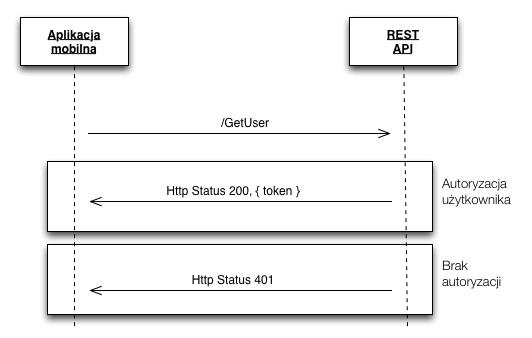
\includegraphics[width=1\linewidth]{assets/auth_schema.png}
		\caption{Schemat autoryzacji użytkownika}
	\label{fig:auth_schema}
\end{figure}

\newpage

\subsection{Synchronizacja treningów} % (fold)
\label{sub:synchronizacja_trening_w}
\paragraph{} % (fold)
\label{par:}
W celu umożliwienia użytkownikowi zarządzania treningami, nagranymi za pomocą aplikacji mobilnej, w serwisie internetowym web serwis posiada metody pozwalające na przesyłanie danych z urządzenia na serwer. Proces synchronizacji polega na wysłaniu dwóch rządań. Pierwszego w celu stworzenia nowego treningu w bazie na serwerze i wygenerowaniu jego unikalnego identyfikatora. Drugiego przesyłającego pozycje zczytane z GPS, jeżeli takowe zostały zapisane w pamięci telefonu. Celem rozdzielenia tych dwóch procesów jest zapewnienie w przyszłości możliwości wysyłania pozycji GPS w paczkach. Pozwoli to na zmniejszenie ryzyka utraty danych oraz ułatwi proces retransmisji danych, które nie zostały zapisane w bazie danych na serwerze. Szczegółowe parametry dotyczące wysyłanych rządań przedstawione zsotały w tabelach 5.2 i 5.3 .

\begin{figure}[ht]
	\centering
		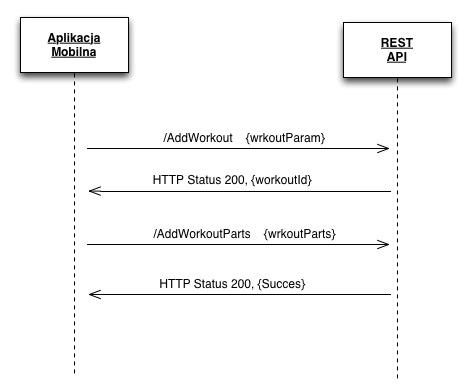
\includegraphics[width=1\linewidth]{assets/workout_parts.png}
		\caption{Schemat synchronizacji treningów}
	\label{fig:workout_parts}
\end{figure}

\begin{table}
 \label{workout}
  \caption{Tworzenie treningu na serwerze}
  \begin{center}
  \begin{tabular}{| l | l |}
  	\hline
  	Metoda & POST \\ \hline
  	URI & http://runner.jacbar.pl/Api.svc/AddWorkout \\ \hline
  	Autoryzacja & token \\ \hline
  	HTTP Status & 200 - ok \\
                & 401 - brak autoryzacji \\
                & 400 - nieprawidłowe rządanie \\ \hline
    Przykładowe dane & \{ \\
    								 & \quad ''Distance'' : ''2000'', \\
    								 & \quad ''Duration" : ''300'', \\
    								 & \quad ''Start'' : ''2012-12-03 23:45:00'', \\
    								 & \quad ''End'' : ''2012-03-12 23:59:00'', \\
    								 & \quad ''Type'' : ''1'' \\ 
    								 & \} \\ \hline
    Przykładowa odpowiedź & \{ \\
                          & \quad ''workoutId'' : ''5'' \\
                          & \} \\ \hline
  \end{tabular}
  \end{center}
\end{table}


\begin{table}
 \label{workoutpart}
  \caption{Synchronizacja zarejestrowanych współrzędnych geograficznych}
  \begin{center}
  \begin{tabular}{| l | l |}
  	\hline
  	Metoda & POST \\ \hline
  	URI & http://runner.jacbar.pl/Api.svc/AddWorkoutParts \\ \hline
  	Autoryzacja & token\\ \hline
  	HTTP Status & 200 - ok \\
                & 401 - brak autoryzacji \\
                & 400 - nieprawidłowe rządanie \\ \hline
    Przykładowe dane & \{ \\
    								 & \quad ''WorkoutId'' : ''5'', \\
    								 & \quad ''WorkoutParts'' : [ \\
    								 & \qquad \{ \\
    								 & \quad \qquad ''Latitiude'' : ''51.09309479832'', \\
    								 & \quad \qquad ''Longitude'' : ''51.09309479832'', \\
    								 & \quad \qquad ''Date'' : ''2012-03-12 23:57:00'' \\
    								 & \qquad \}, \\    								 & \qquad \{ \\
    								 & \quad \qquad ''Latitiude'' : ''51.09309479832'', \\
    								 & \quad \qquad ''Longitude'' : ''51.09309479832'', \\
    								 & \quad \qquad ''Date'' : ''2012-03-12 23:57:10'' \\
    								 & \qquad \} \\
    								 & \quad ] \\
    								 & \} \\ \hline
    Przykładowa odpowiedź & \{ \\
                          & \quad ''Success'' : ''true'' \\
                          & \} \\ \hline
  \end{tabular}
  \end{center}
\end{table}

